\documentclass[problem]{mcs}

\begin{pcomments}
  \pcomment{CP_2_layer_array_network}
  \pcomment{from: S09.final}
\end{pcomments}

\pkeywords{
  networks
  congestion
  routing
}

%%%%%%%%%%%%%%%%%%%%%%%%%%%%%%%%%%%%%%%%%%%%%%%%%%%%%%%%%%%%%%%%%%%%%
% Problem starts here
%%%%%%%%%%%%%%%%%%%%%%%%%%%%%%%%%%%%%%%%%%%%%%%%%%%%%%%%%%%%%%%%%%%%%

\begin{problem}
  The $n$-input \emph{\idx{2-D Array}} network was shown to have
  congestion 2.  An $n$-input \term{2-Layer Array} consisting of two
  $n$-input 2-D Arrays connected as pictured below for $n=4$.

  \begin{center}
  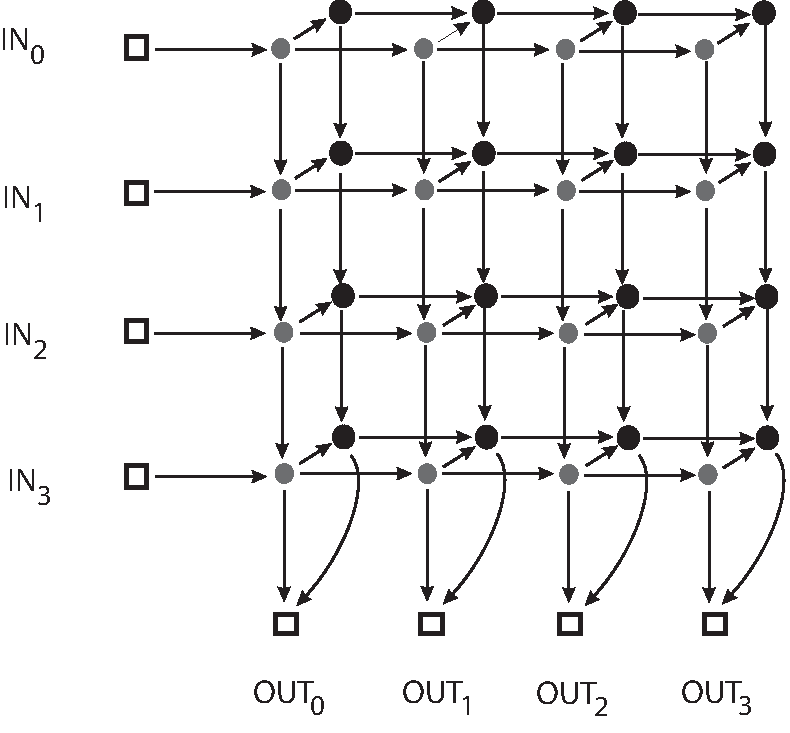
\includegraphics[width=2.25in,clip]{2-layer-grid-new}
  \end{center}

  In general, an $n$-input 2-Layer Array has two layers of switches, with
  each layer connected like an $n$-input 2-D Array.  There is also an edge from
  each switch in the first layer to the corresponding switch in the second
  layer.  The inputs of the 2-Layer Array  enter the left side of the first
  layer, and the $n$ outputs leave from the bottom row of either layer.

  \bparts

  \ppart For any given input-output permutation, there is a way to route
  packets that achieves congestion 1.  Describe how to route the packets in 
  this way.

  \begin{solution}
     To route a packet from input $i$ to output $j$, use
    the path from input $i$ to the right along row $i$ of the input layer
    until column $j$.  Then take the edge to the corresponding switch in
    column $j$ of the output layer, and continue the path downward along
    column $j$ in the output layer to output $j$.  Now each packet moves to
    the right in its own row of the input layer and down in its own column
    in the output layer, and so packets never cross.  That is, congestion is
    1.
  \end{solution}

  \ppart What is the latency of a routing designed to minimize latency?

\begin{solution}
    Latency is minimized over all permutations by routing using shortest
    paths, and a shortest path routing must stick exclusively to the first
    layer.  Thus the latency of a routing designed to minimize latency is
    the same as the latency of the 2D-array: $2n$.
\end{solution}

  \ppart Explain why the congestion of any minimum latency (CML) routing 
    of packets through this network is greater than the network's congestion.

\begin{solution}
If we want minimum latency, we will never leave 
    the input layer, as any path from input to output including the second 
    layer could be done instead entirely on the input layer in less time.  
    This makes the problem reduce to a standard 2D grid, which we know has 
    congestion 2.
\end{solution}

  \eparts
\end{problem}

\endinput
